\documentclass{article}

\usepackage[english]{babel}
\usepackage[utf8]{inputenc}
\usepackage{amsmath}
\usepackage{amsthm}
\usepackage{amssymb}
\usepackage{mathtools}
\usepackage{amsfonts}
\usepackage{subcaption}
\usepackage{graphicx}
\usepackage{wrapfig}
\usepackage{bbm}
\usepackage{dsfont}
\usepackage{listings}

% set up margin
\usepackage
[
  a4paper,
  left=3cm,
  right=3cm,
  top=3cm,
  bottom=3cm,
]
{geometry}

% set up header
\usepackage{fancyhdr}
\pagestyle{fancy}
\fancyhf{}
\lhead{6.438 Algorithms for Inference}
\chead{Problem Set 3}
\rhead{Hongzi Mao}
\cfoot{\thepage}
\rfoot{\footnotesize{\emph{Collaborated with: Hongzhou Ye, Zhiwei Ding}}}

% footer line
\renewcommand{\footrulewidth}{0.4pt}

% sans serif italic
\newcommand{\s}[1]{\textsf{\textit{#1}}}

% bold face sans serif
\newcommand{\bs}[1]{\textsf{\textbf{#1}}}

% set symbol
\usepackage[mathscr]{euscript}

% empty set
\let\emptyset\varnothing

% qed
\newcommand{\qeds}{\hfill\qedsymbol}

% math bold face
\newcommand{\bm}{\mathbf}

% argmax
\DeclareMathOperator*{\argmax}{argmax}

% independence symbol
\makeatletter
\newcommand*{\indep}{%
  \mathbin{%
    \mathpalette{\@indep}{}%
  }%
}
\newcommand*{\nindep}{%
  \mathbin{%                   % The final symbol is a binary math operator
    \mathpalette{\@indep}{\not}% \mathpalette helps for the adaptation
                               % of the symbol to the different math styles.
  }%
}
\newcommand*{\@indep}[2]{%
  \sbox0{$#1\perp\m@th$}%        box 0 contains \perp symbol
  \sbox2{$#1=$}%                 box 2 for the height of =
  \sbox4{$#1\vcenter{}$}%        box 4 for the height of the math axis
  \rlap{\copy0}%                 first \perp
  \dimen@=\dimexpr\ht2-\ht4-.2pt\relax
  \kern\dimen@
  {#2}
  \kern\dimen@
  \copy0 %                       second \perp
} 
\makeatother

%%%%%%%%%%%%%%%%%%%%%%%%%%%%%%%%%%%%%%%%%%%%%%%%%%%%%%%%%%%%%%%%%%%%%%%%
%%%%%%%%%%%%%%%%%%%%%%%%% Begin document here %%%%%%%%%%%%%%%%%%%%%%%%%%
%%%%%%%%%%%%%%%%%%%%%%%%%%%%%%%%%%%%%%%%%%%%%%%%%%%%%%%%%%%%%%%%%%%%%%%%
\begin{document}
 
\section*{Problem 3.1}
%
(a) When marginalizing Gaussian variables, the variance term carries from the joint covariance.
As a result, for variables $\s{x}_i, \s{x}_j$ with no connection on covariance graph, the covariance
matrix has $0$ on all entries off the diagonal. Therefore, all unconditional independencies are
%$\begin{bmatrix}
%    \Lambda_{ii} & 0 \\
%    0 & \Lambda_{ij}
%\end{bmatrix}$. 
\begin{equation*}
	\s{x}_1 \indep \s{x}_3, \; \s{x}_1 \indep \s{x}_4,\; \s{x}_2 \indep \s{x}_4.
\end{equation*}
The corresponding covariance matrix is
$\bm{\Lambda} = \begin{bmatrix}
    \Lambda_{11} & \Lambda_{12} & 0 & 0 \\
    \Lambda_{21} & \Lambda_{22} & \Lambda_{23} & 0 \\
    0 & \Lambda_{32} & \Lambda_{33} & \Lambda_{34} \\
    0 & 0 & \Lambda_{43} & \Lambda_{44}
\end{bmatrix}$. Thus, in general, the information matrix $\bm{J} = \bm{\Lambda}^{-1}$ has
non-zero values for all entries. In order words, the undirected graph is fully connected.
Hence, there is no conditional independencies.
\\
\\


\noindent
(b) To abuse the notation, we use $\bm{\Lambda}_{i,j,\cdots,k}$ to indicate the covariance matrix of variables $\s{x}_i, \s{x}_j, \cdots, \s{x}_k$. Thus, the covariance matrix for $\s{x}_1, \s{x}_2, \s{x}_3, \s{x}_4$ is
$\bm{\Lambda}_{1, 2, 3, 4} = \begin{bmatrix}
    \Lambda_{11} & 0 & \Lambda_{13} & 0 \\
    0 & \Lambda_{22} & 0 & \Lambda_{24} \\
    \Lambda_{31} & 0 & \Lambda_{33} & 0 \\
    0 & \Lambda_{42} & 0 & \Lambda_{44}
\end{bmatrix}$, and the corresponding covariance graph is shown in Figure~\ref{f:1b}.
\begin{figure}[h]
  \centering
  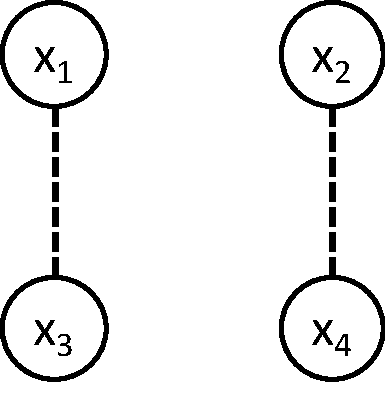
\includegraphics[width=0.2\columnwidth]{1b.pdf}
    \vspace{-0.1cm}
  \caption{Covariance graph with the fewest possible edges for $p_{\s{x}_1, \s{x}_2, \s{x}_3, \s{x}_4}$.}
  \label{f:1b}
\end{figure}
\\
\\

\noindent
(c) Notice that $\bm{\Lambda}_{5,6} =
\begin{bmatrix}
    \Lambda_{55} & 0 \\
    0 & \Lambda_{66}
\end{bmatrix}$
%
and
%
$\bm{\Lambda}_{(5,6), (1,2,3,4)} = \bm{\Lambda}_{(1,2,3,4), (5,6)}^T =
\begin{bmatrix}
    \Lambda_{51} & \Lambda_{52} & 0 & 0 \\
    0 & 0 & \Lambda_{63} & \Lambda_{64}
\end{bmatrix}$. Thus, 
$\bm{\Lambda}_{(1,2,3,4), (5,6)}\bm{\Lambda}_{5,6}^{-1} \bm{\Lambda}_{(5,6), (1,2,3,4)}
\simeq
\begin{bmatrix}
    * & * & 0 & 0 \\
    * & * & 0 & 0 \\
    0 & 0 & * & * \\
    0 & 0 & * & *
\end{bmatrix}$,
where ``$*$'' denotes non-zero values. Hence, the covariance matrix for
$\s{x}_1, \s{x}_2, \s{x}_3, \s{x}_4 | \s{x}_5, \s{x}_6$ \,is\;
$\bm{\Lambda}_{(1,2,3,4)} + \bm{\Lambda}_{(1,2,3,4), (5,6)}\bm{\Lambda}_{5,6}^{-1} \bm{\Lambda}_{(5,6), (1,2,3,4)}
\simeq
\begin{bmatrix}
    * & * & * & 0 \\
    * & * & 0 & * \\
    * & 0 & * & * \\
    0 & * & * & *
\end{bmatrix}$.
The corresponding covariance graph is shown in Figure~\ref{f:1c}.
\begin{figure}[h]
  \centering
  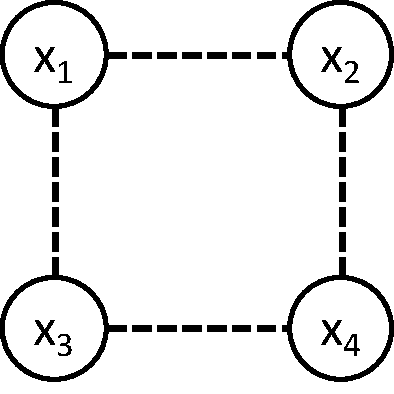
\includegraphics[width=0.2\columnwidth]{1c.pdf}
    \vspace{-0.1cm}
  \caption{Covariance graph with the fewest possible edges for
  $p_{\s{x}_1, \s{x}_2, \s{x}_3, \s{x}_4|\s{x}_5, \s{x}_6}$.}
  \label{f:1c}
\end{figure}
\pagebreak

%%%%%%%%%%%%%%%%%%%%%%%%%%%%%%%%%%%%%%%%%%%%%%%%%%%%%%%%%%%%%%%%%%%%%%%%%%%%%%%%%%%%%%%%
\section*{Problem 3.2}
(a) Suppose $\bs{x}_1$ and $\bs{z}$ are independent and their information matrix is
$\bm{J}' =
\begin{bmatrix}
    \bm{J}_{11}' & 0 \\
    0 & \bm{J}_{22}'
\end{bmatrix}$, potential vector is $[\bm{h}_1'\,^T, \bm{h}_2'\,^T]\,^T$. Now,
\begin{align*}
p_{\bs{x}_1, \bs{x}_2}(\bm{x}_1, \bm{x}_2) &= 
p_{\bs{x}_1, \bs{z}}(\bm{x}_1, \bm{x}_2 + \bm{A}\bm{x}_1) \\
&\propto
\exp\left\{ -\frac{1}{2}
\begin{bmatrix}
    \bm{x}_1^T & \bm{x}_2^T + \bm{x}_1^T \bm{A}^T
\end{bmatrix}
\begin{bmatrix}
    \bm{J}_{11}' & 0 \\
    0 & \bm{J}_{22}'
\end{bmatrix}
\begin{bmatrix}
    \bm{x}_1 \\
    \bm{x}_2 + \bm{A}\bm{x}_1
\end{bmatrix} + 
\begin{bmatrix}
    \bm{h}_1'^T & \bm{h}_2'^T
\end{bmatrix}
\begin{bmatrix}
    \bm{x}_1 \\
    \bm{x}_2 + \bm{A}\bm{x}_1
\end{bmatrix}
\right\}\\
&\propto \exp \bigg[
-\frac{1}{2}\left(
\bm{x}_1^T\bm{J}_{11}'\bm{x}_1 +
\bm{x}_2^T\bm{J}_{22}'\bm{x}_2 +
\bm{x}_2^T\bm{J}_{22}'\bm{A}\bm{x}_1 +
\bm{x}_1^T\bm{A}^T\bm{J}_{22}'\bm{x}_2 +
\bm{x}_1^T\bm{A}^T\bm{J}_{22}'\bm{A}\bm{x}_1
\right) \\
&\;\;\;\;\;+ \bm{h}_1'^T \bm{x}_1
+ \bm{h}_2'^T \bm{x}_2
+ \bm{h}_2'^T \bm{A}\bm{x}_1 \bigg].
\end{align*}
%
Meanwhile, 
%
\begin{align*}
p_{\bs{x}_1, \bs{x}_2}(\bm{x}_1, \bm{x}_2) &\propto \exp\left\{ -\frac{1}{2}
\begin{bmatrix}
    \bm{x}_1^T & \bm{x}_2^T 
\end{bmatrix}
\begin{bmatrix}
    \bm{J}_{11} & \bm{J}_{12} \\
    \bm{J}_{21} & \bm{J}_{22}
\end{bmatrix}
\begin{bmatrix}
    \bm{x}_1 \\
    \bm{x}_2
\end{bmatrix} + 
\begin{bmatrix}
    \bm{h}_1^T & \bm{h}_2^T
\end{bmatrix}
\begin{bmatrix}
    \bm{x}_1 \\
    \bm{x}_2
\end{bmatrix}
\right\}\\
&\propto\exp\left[
-\frac{1}{2}\left(
\bm{x}_1^T\bm{J}_{11}\bm{x}_1 +
\bm{x}_1^T\bm{J}_{12}\bm{x}_2 +
\bm{x}_2^T\bm{J}_{21}\bm{x}_1 +
\bm{x}_2^ T\bm{J}_{22}'\bm{x}_2
\right) + 
\bm{h}_1^T \bm{x}_1 +
\bm{h}_2^T \bm{x}_2
\right].
\end{align*}
%
Thus, by term matching,
%
\begin{align*}
	\bm{J}_{22}' &= \bm{J}_{22}, \\
	\bm{J}_{22}'\bm{A} &= \bm{J}_{21} \implies \bm{A} = \bm{J}_{22}^{-1}\bm{J}_{21}, \\
	\bm{J}_{11}' + \bm{A}^T\bm{J}_{22}'\bm{A} &= \bm{J}_{11},\\ % \implies \bm{J}_{11}' = \bm{J}_{11} - \bm{A}^T\bm{J}_{22}\bm{A}, \\
	\bm{h}_2' &= \bm{h}_2,\\
	\bm{h}_1' &= \bm{h}_1 - \bm{A}^T\bm{h}_2.
\end{align*}
Since $\bs{x}_1$ and $\bs{z}$ are independent, $\bs{x}_1 \sim \mathscr{N}^{-1}(\bm{J}_{11}', \bm{h}_{1}')$.
By plugging in $\bm{A} = \bm{J}_{22}^{-1}\bm{J}_{21}$ from above, and knowing
$\bm{J}_{11}$ and $\bm{J}_{22}$ being symmetric, and $\bm{J}_{12}^T =\bm{J}_{21}$, we have
\begin{align*}
	\bm{J}_{11}' &= \bm{J}_{11} - \bm{A}^T\bm{J}_{22}\bm{A} = \bm{J}_{11} - \bm{J}_{12}\bm{J}_{22}^{-1}\bm{J}_{21},\\
	\bm{h}_1' &= \bm{h}_1 - \bm{J}_{12}\bm{J}_{22}^{-1}\bm{h}_2.
\end{align*}

\noindent
(b) Let
\begin{align*}
\begin{bmatrix}
    \bm{J}_{11} & \bm{J}_{12} \\
    \bm{J}_{21} & \bm{J}_{22}
\end{bmatrix}
\begin{bmatrix}
    \bm{m}_{1}\\
    \bm{m}_{2}
\end{bmatrix} = 
\begin{bmatrix}
    \bm{h}_{1}\\
    \bm{h}_{2}
\end{bmatrix},
\end{align*}
which brings
\begin{align*}
	&\bm{J}_{11}\bm{m}_1 + \bm{J}_{12}\bm{m}_2 = \bm{h}_1\\
	&\bm{J}_{21}\bm{m}_1 + \bm{J}_{22}\bm{m}_2 = \bm{h}_2.
\end{align*}
%
From the second equation above, we have
\begin{align*}
	\bm{m}_2 = \bm{J}_{22}^{-1}(\bm{h}_2 - \bm{J}_{21}\bm{m}_1).
\end{align*}
%
Plugging in the first equation,
\begin{align*}
	\bm{J}_{11}\bm{m}_1 + \bm{J}_{12}\bm{J}_{22}^{-1}(\bm{h}_2 - \bm{J}_{21}\bm{m}_1) = \bm{h}_1.
\end{align*}
Rearranging,
\begin{align*}
	\left(\bm{J}_{11} + \bm{J}_{12}\bm{J}_{22}^{-1}\bm{J}_{21}\right)\bm{m}_1 = \bm{h}_1 - \bm{J}_{12}\bm{J}_{22}^{-1}\bm{h}_2.
\end{align*}
\\

\noindent
(c)(i) Notice that
\begin{align*}
p_{\bs{x}_1, \bs{x}_2, \bs{x}_3}(\bm{x}_1, \bm{x}_2, \bm{x}_3) &\propto	
\exp\left\{-\frac{1}{2}\left(
\begin{bmatrix}
    \bm{x}_1^T & \bm{x}_2^T & \bm{x}_3^T 
\end{bmatrix}
\begin{bmatrix}
    \bm{J}_{11} & \bm{J}_{12} & \bm{J}_{13}\\
    \bm{J}_{21} & \bm{J}_{22} & 0 \\
    \bm{J}_{31} & 0 & \bm{J}_{33}\\
\end{bmatrix}
\begin{bmatrix}
    \bm{x}_1 \\
    \bm{x}_2 \\
    \bm{x}_3
\end{bmatrix}\right) + 
\begin{bmatrix}
    \bm{h}_1^T & \bm{h}_2^T & \bm{h}_3^T
\end{bmatrix}
\begin{bmatrix}
    \bm{x}_1 \\
    \bm{x}_2 \\
    \bm{x}_3
\end{bmatrix}
\right\} \\
&\propto \exp\bigg[-\frac{1}{2}\left(
\bm{x}_1^T\bm{J}_{11}\bm{x}_1 +
\bm{x}_1^T\bm{J}_{12}\bm{x}_2 +
\bm{x}_1^T\bm{J}_{13}\bm{x}_3 +
\bm{x}_2^T\bm{J}_{21}\bm{x}_1 +
\bm{x}_2^T\bm{J}_{22}\bm{x}_2 +
\bm{x}_3^T\bm{J}_{31}\bm{x}_3 +
\bm{x}_3^T\bm{J}_{33}\bm{x}_3
\right)\\
&\;\;\;\; + \bm{h}_1^T\bm{x}_1 + \bm{h}_2^T\bm{x}_2 + \bm{h}_3^T\bm{x}_3 \bigg] \\
&\propto \underbrace{\exp\left[-\frac{1}{2}\left(
\bm{x}_1^T\bm{J}_{11}\bm{x}_1 +
\bm{x}_1^T\bm{J}_{12}\bm{x}_2 +
\bm{x}_2^T\bm{J}_{21}\bm{x}_1 +
\bm{x}_2^T\bm{J}_{22}\bm{x}_2
\right) + \bm{h}_1^T\bm{x}_1 + \bm{h}_2^T\bm{x}_2
\right]}_{h(\bm{x}_1, \bm{x}_2)}\\
&\times \underbrace{\exp\left[-\frac{1}{2}\left(
\bm{x}_1^T\bm{J}_{13}\bm{x}_3 +
\bm{x}_3^T\bm{J}_{31}\bm{x}_3 +
\bm{x}_3^T\bm{J}_{33}\bm{x}_3
\right) + \bm{h}_3^T\bm{x}_3 \right]}_{g(\bm{x}_1, \bm{x}_3)}.
\end{align*}

Hence,
%
$\bs{x}_2 \indep \bs{x}_3 \,|\, \bs{x}_1.$ \qeds
\\

\noindent
(ii) Directly using equation (2), we have
\begin{align*}
	\bm{J}_b &= \bm{J}_{11} -
\begin{bmatrix}
    \bm{J}_{12} & \bm{J}_{13} 
\end{bmatrix}
\begin{bmatrix}
    \bm{J}_{22} & 0 \\
    0 & \bm{J}_{33}
\end{bmatrix}^{-1}
\begin{bmatrix}
    \bm{J}_{21} \\
    \bm{J}_{31}
\end{bmatrix} \\
&= \bm{J}_{11} -
\begin{bmatrix}
    \bm{J}_{12} & \bm{J}_{13} 
\end{bmatrix}
\begin{bmatrix}
    \bm{J}_{22}^{-1} & 0 \\
    0 & \bm{J}_{33}^{-1}
\end{bmatrix}
\begin{bmatrix}
    \bm{J}_{21} \\
    \bm{J}_{31}
\end{bmatrix}\\
&= \bm{J}_{11} - \bm{J}_{12}\bm{J}_{22}^{-1}\bm{J}_{21} - \bm{J}_{13}\bm{J}_{33}^{-1}\bm{J}_{31},
\end{align*}
and
\begin{align*}
	\bm{h}_b &= \bm{h}_1 - 
\begin{bmatrix}
    \bm{J}_{12} & \bm{J}_{13} 
\end{bmatrix}
\begin{bmatrix}
    \bm{J}_{22} & 0 \\
    0 & \bm{J}_{33}
\end{bmatrix}^{-1}
\begin{bmatrix}
    \bm{h}_{2} \\
    \bm{h}_{3}
\end{bmatrix} \\
&= \bm{h}_1 - 
\begin{bmatrix}
    \bm{J}_{12} & \bm{J}_{13} 
\end{bmatrix}
\begin{bmatrix}
    \bm{J}_{22}^{-1} & 0 \\
    0 & \bm{J}_{33}^{-1}
\end{bmatrix}
\begin{bmatrix}
    \bm{h}_{2} \\
    \bm{h}_{3}
\end{bmatrix} \\
&=\bm{J}_{11} - \bm{J}_{12}\bm{J}_{22}^{-1}\bm{h}_{2} - \bm{J}_{13}\bm{J}_{33}^{-1}\bm{h}_{3}.
\end{align*}\qeds
\pagebreak

%%%%%%%%%%%%%%%%%%%%%%%%%%%%%%%%%%%%%%%%%%%%%%%%%%%%%%%%%%%%%%%%%%%%%%%%%%%%%%%%%%%%%%%%
\section*{Problem 3.3}
(a) Since $\bs{y} = \bm{C}\bs{x} + \bs{v}$, we have
\begin{align*}
p_{\bs{x}, \bs{y}}(\bm{x}, \bm{y}) &=
P_{\bs{x}\sim\mathscr{N}^{-1}(\bm{h}_x, \bm{J}_x)}(\bm{x})P_{\bs{y}-\bm{C}\bs{x}
=\bs{v}\sim\mathscr{N}(0,\bm{R})}(\bm{y}-\bm{C}\bm{x})\\
&\propto\exp\left[-\frac{1}{2}\bm{x}^T\bm{J}_{\bs{x}}\bm{x}+\bm{h}_\bs{x}^T\bm{x}\right]
\exp\left[-\frac{1}{2}(\bm{y}-\bm{C}\bm{x})^T\bm{R}(\bm{y}-\bm{C}\bm{x})\right]\\
&\propto\exp\left[-\frac{1}{2}\bm{x}^T\bm{J}_{\bs{x}}\bm{x}+\bm{h}_\bs{x}^T\bm{x}\right]
\exp\left[-\frac{1}{2}(\bm{y}^T\bm{R}\bm{y} - \bm{y}^T\bm{R}\bm{C}\bm{x} - \bm{x}^T\bm{C}^T\bm{R}\bm{y}
+ \bm{x}^T\bm{C}^T\bm{R}\bm{C}\bm{x})\right]\\
&\propto\exp\left[-\frac{1}{2}\big(
\bm{x}^T(\bm{J}_\bs{x}+\bm{C}^T\bm{R}\bm{C})\bm{x}
- \bm{y}^T\bm{R}\bm{C}\bm{x}
-\bm{x}^T\bm{C}^T\bm{R}\bm{y}
+\bm{y}^T\bm{R}\bm{y}\big)
+ \bm{h}_\bs{x}^T\bm{x}\right]\\
& = \exp\left\{
-\frac{1}{2}
\begin{bmatrix}
    \bm{x}^T & \bm{y}^T
\end{bmatrix}
\begin{bmatrix}
    \bm{J}_\bs{x}+\bm{C}^T\bm{R}\bm{C} & -\bm{C}^T\bm{R} \\
    -\bm{R}\bm{C} & \bm{R}
\end{bmatrix}
\begin{bmatrix}
    \bm{x} \\
    \bm{y}
\end{bmatrix}
+ 
\begin{bmatrix}
    \bm{h}_{\bs{x}}^T & \bm{0}
\end{bmatrix}
\begin{bmatrix}
    \bm{x} \\
    \bm{y}
\end{bmatrix}
\right\}.
\end{align*}
Therefore, the information matrix and potential vector for $p_{\bs{x}, \bs{y}}(\bm{x}, \bm{y})$ are
\begin{align*}
	\bm{J}_{\bs{x}, \bs{y}} = \begin{bmatrix}
    \bm{J}_\bs{x}+\bm{C}^T\bm{R}\bm{C} & -\bm{C}^T\bm{R} \\
    -\bm{R}\bm{C} & \bm{R}
\end{bmatrix},\;\;\;
\bm{h}_{\bs{x}, \bs{y}} = 
\begin{bmatrix}
    \bm{h}_{\bs{x}} \\
    \bm{0}
\end{bmatrix}.
\end{align*}
Using the conditional derivation of information matrix and potential vector on $p_{\bs{x}|\bs{y}}(\bm{x}| \bm{y})$, we have
\begin{align*}
	\bm{J}_{\bs{x}|\bs{y}} = \bm{J}_\bs{x}+\bm{C}^T\bm{R}\bm{C},
\end{align*}
and
\begin{align*}
	\bm{h}_{\bs{x}|\bs{y}} = \bm{h}_{\bs{x}} - (-\bm{C}^T\bm{R})\bm{y} = \bm{h}_{\bs{x}} + \bm{C}^T\bm{R}\bm{y}.
\end{align*}
\\

\noindent
(b) since $\s{y}_1 = \s{x}_1 + \s{v}_1$ and $\s{y}_2 = \s{x}_3 + \s{v}_2$, we have
\begin{align*}
\begin{bmatrix}
    \bm{y}_{1}\\
    \bm{y}_{2}
\end{bmatrix} = 
\begin{bmatrix}
    1 & 0 & 0 & 0 \\
    0 & 0 & 1 & 0
\end{bmatrix}
\begin{bmatrix}
    \bm{x}_{1}\\
    \bm{x}_{2}\\
    \bm{x}_{3}\\
    \bm{x}_{4}
\end{bmatrix} + 
\begin{bmatrix}
    \bm{v}_{1}\\
    \bm{v}_{2}
\end{bmatrix}.
\end{align*}
%

Thus, $\bm{C} =
\begin{bmatrix}
    1 & 0 & 0 & 0 \\
    0 & 0 & 1 & 0
\end{bmatrix}$.
%

Plugging in $\bm{C}$, we have $\bm{C}^T\bm{R}\bm{C} = 
\begin{bmatrix}
    1 & 0 & 0 & 0 \\
    0 & 0 & 0 & 0 \\
    0 & 0 & 1 & 0 \\
    0 & 0 & 0 & 0 \\
\end{bmatrix}$. Hence, 
\begin{align*}
\bm{J}_{\bs{x}, \bs{y}} =
\begin{bmatrix}
    J_{11} + 1 & J_{12} & 0 & 0 & -1 & 0\\
    0 & J_{22} & J_{23} & J_{24} & 0 & 0 \\
    0 & J_{32} & J_{33} + 1 & 0 & 0 & -1 \\
    0 & J_{42} & 0 & J_{44} & 0 & 0 \\
    -1 & 0 & 0 & 0 & 1 & 0 \\
    0 & 0 & -1 & 0 & 0 & 1
\end{bmatrix}, \;\;
\bm{h}_{\bs{x}, \bs{y}} = 
\begin{bmatrix}
    h_1 \\
    h_2 \\
    h_3 \\
    h_4 \\
    0 \\
    0\\
\end{bmatrix}.
\end{align*}

Now,
\begin{align*}
	J_{\s{x}_3\to\s{x}_2} &= -J_{23}(J_{33} + 1 + J_{\s{y}_2\to\s{x}_3})^{-1}J_{32},\\
\end{align*}

where 
\begin{align*}
	J_{\s{y}_2\to\s{x}_3} &= 1\times1^{-1}\times -1 = -1.\\
\end{align*}

Hence, 
\begin{align*}
	J_{\s{x}_3\to\s{x}_2} &= -J_{23}J_{33}^{-1}J_{32}.\\
\end{align*}

Similarly,
\begin{align*}
	h_{\s{x}_3\to\s{x}_2} &= -J_{23}(J_{33} + 1 + J_{\s{y}_2\to\s{x}_3})^{-1}(h_3+h_{\s{y}_2\to\s{x}_3}),\\
\end{align*}

where
\begin{align*}
	J_{\s{y}_2\to\s{x}_3} &= 1\times1^{-1}\times -1 = -1.\\
	h_{\s{y}_2\to\s{x}_3} &= 1\times1^{-1}\times 0 = 0.\\
\end{align*}

Hence,
\begin{align*}
	h_{\s{x}_3\to\s{x}_2} &= -J_{23}J_{33}^{-1}h_{3}.\\
\end{align*}
\\

\noindent
(c) Similar to (b), we have $\bm{C} =
\begin{bmatrix}
    1 & 0 & 0 & 0 \\
    0 & 0 & 1 & 0 \\
    0 & 0 & 1 & 0
\end{bmatrix}$, $\bm{C}^T\bm{R}\bm{C} = 
\begin{bmatrix}
    1 & 0 & 0 & 0 \\
    0 & 0 & 0 & 0 \\
    0 & 0 & 2 & 0 \\
    0 & 0 & 0 & 0 \\
\end{bmatrix}$. Thus,
\begin{align*}
\bm{J}_{\bs{x}, \bs{y}} =
\begin{bmatrix}
    J_{11} + 1 & J_{12} & 0 & 0 & -1 & 0 & 0\\
    0 & J_{22} & J_{23} & J_{24} & 0 & 0 & 0\\
    0 & J_{32} & J_{33} + 2 & 0 & 0 & -1 & -1\\
    0 & J_{42} & 0 & J_{44} & 0 & 0 & 0\\
    -1 & 0 & 0 & 0 & 1 & 0 & 0\\
    0 & 0 & -1 & 0 & 0 & 1 & 0\\
    0 & 0 & -1 & 0 & 0 & 0 & 1\\
\end{bmatrix}, \;\;
\bm{h}_{\bs{x}, \bs{y}} = 
\begin{bmatrix}
    h_1 \\
    h_2 \\
    h_3 \\
    h_4 \\
    0 \\
    0\\
    0\\
\end{bmatrix}.
\end{align*}

Since $J_{\s{y}_3\to\s{x}_3} = J_{\s{y}_2\to\s{x}_3} = -1$
and $h_{\s{y}_3\to\s{x}_3} = h_{\s{y}_2\to\s{x}_3} = 0$, we have
\begin{align*}
	J_{\s{x}_3\to\s{x}_2} &= -J_{23}(J_{33} + 2 + 
	J_{\s{y}_2\to\s{x}_3} + J_{\s{y}_3\to\s{x}_3})^{-1}J_{32}\\
	& = -J_{23}(J_{33} + 2 -1 -1)^{-1}J_{32}\\
	& = -J_{23}J_{33}^{-1}J_{32},
\end{align*}

and
\begin{align*}
	h_{\s{x}_3\to\s{x}_2} &= -J_{23}J_{33} + 2 + 
	J_{\s{y}_2\to\s{x}_3} + J_{\s{y}_3\to\s{x}_3})^{-1}
	(h_3+h_{\s{y}_2\to\s{x}_3} + h_{\s{y}_3\to\s{x}_3}),\\
	&= -J_{23}J_{33} + 2 + 
	-1 -1)^{-1}
	(h_3+0 + 0),\\
	&=-J_{23}J_{33}^{-1}h_{3}.
\end{align*}
\pagebreak

%%%%%%%%%%%%%%%%%%%%%%%%%%%%%%%%%%%%%%%%%%%%%%%%%%%%%%%%%%%%%%%%%%%%%%%%%%%%%%%%%%%%%%%%
\section*{Problem 3.4}
(a) Note that
\begin{align*}
	p_{\s{x}_a}(\s{x}_a = 0) &\propto \sum_{x_b}\psi_{ab}(0, x_b) = \psi_{ab}(0, 0) +  \psi_{ab}(0, 1) = 1 + 10 = 11,\\
	p_{\s{x}_a}(\s{x}_a = 1) &\propto \sum_{x_b}\psi_{ab}(1, x_b) = \psi_{ab}(1, 0) +  \psi_{ab}(1, 1) = 1 + 10 = 11.
\end{align*}

Similarly, $p_{\s{x}_b}(\s{x}_b = 0) = p_{\s{x}_b}(\s{x}_b = 1) = 11$. Therefore, there is no unique maximizing value for each variable's marginal.

Now, if we independently choosing the maximizing values for each variable, we could choose $x_a=0$ and $x_b=0$, resulting in a minimum joint probability $p_{\s{x}_a, \s{x}_b}(0,0) \propto 1$, which does not lead to the maximum of the joint distribution. \qeds
\\

\noindent
(b) Let $x_a^*$ be the maximizing value for $\s{x}_a$, that is
\begin{align*}
	x_a^* = \argmax_{x_a} \left[\max_{\bs{x}\backslash\{\s{x}_a\}}p_{\bs{x}}(\bm{x}) \right].
\end{align*}
%

Now, we can use edge max-marginal to determine $x_b^*$ using
\begin{align*}
	x_b^* = \argmax_{x_b} \bigg[\bar{p}_{ab}(x_a^*, x_b)\bigg].
\end{align*}
%

Here, $x_a^*$ and $x_b^*$ together maximize the joint probability as $\bar{p}_{ab}(x_a^*, x_b^*) = \max_{x}p_\s{x}(x)$. This is true because otherwise we could have taken the $x_b$ in $\max_{\bs{x}\backslash\{\s{x}_a\}}p_{\bs{x}}(\bm{x})$ when obtaining $x_a^*$ to get a larger edge max-marginal, resulting in a contradiction. 
\pagebreak

%%%%%%%%%%%%%%%%%%%%%%%%%%%%%%%%%%%%%%%%%%%%%%%%%%%%%%%%%%%%%%%%%%%%%%%%%%%%%%%%%%%%%%%%
\section*{Computational Exercise 1(a) Genetics}
The sum product algorithm implementation is 
\lstset{language=Python}
\lstset{frame=lines}
\lstset{caption={Python implementation of parallel sum product algorithm}}
\lstset{label={code:bp}}
\lstset{basicstyle=\footnotesize}
\begin{lstlisting}
import numpy as np


def ep(edge_potential, i, j, var_i, var_j):
    if (i, j) in edge_potential:
        return edge_potential[(i, j)][var_i, var_j]
    elif (j, i) in edge_potential:
        return edge_potential[(j, i)][var_j, var_i]
    else:
        return None


def get_msg(i, j, node_potential, edge_potential, messages, neighbors):
    # get msg_{i->j}(var)
    distant_msg = {0: 1, 1: 1}
    for k in neighbors[i]:
        if k != j:
            distant_msg[0] *= messages[(k, i)][0]
            distant_msg[1] *= messages[(k, i)][1]

    msg = {}
    msg[0] = node_potential[i][0] * ep(edge_potential, i, j, 0, 0) * distant_msg[0] \
           + node_potential[i][1] * ep(edge_potential, i, j, 1, 0) * distant_msg[1]
    msg[1] = node_potential[i][0] * ep(edge_potential, i, j, 0, 1) * distant_msg[0] \
           + node_potential[i][1] * ep(edge_potential, i, j, 1, 1) * distant_msg[1]

    return msg


def normalize_marginals(marginals):
    for node in marginals:
        p_sum = marginals[node][0] + marginals[node][1]
        marginals[node][0] /= p_sum
        marginals[node][1] /= p_sum


def belief_propagation(node_potential, edge_potential, diameter=np.inf):
    '''
    node_potential: {i -> node_potential}
    edge_potential: {(i, j) -> edge_potential}
    output: {i -> marginal}
    '''
    
    # find neighbor nodes for each node
    neighbors = {}
    for i in node_potential:
        neighbors[i] = set()
    for (i, j) in edge_potential:
        neighbors[i].add(j)
        neighbors[j].add(i)

    # initialize random message
    messages = {}
    init_msg = {0: 1, 1: 1}
    for (i, j) in edge_potential:
        messages[(i, j)] = init_msg
        messages[(j, i)] = init_msg

    d = min(diameter, len(node_potential))

    # tree diameter <= total number of nodes
    for _ in range(d):
        new_messages = {}
        for i in node_potential:
            for j in neighbors[i]:
                msg = get_msg(
                    i, j,
                    node_potential,
                    edge_potential,
                    messages,
                    neighbors)
                new_messages[(i, j)] = msg
        assert len(new_messages) == len(messages)
        messages = new_messages

    # compute marginals
    marginals = {}
    for i in node_potential:
        marginals[i] = {}
        msg = {0: 1, 1: 1}
        for j in neighbors[i]:
            msg[0] *= messages[(j, i)][0]
            msg[1] *= messages[(j, i)][1]
        marginals[i][0] = node_potential[i][0] * msg[0]
        marginals[i][1] = node_potential[i][1] * msg[1]

    # normalize marginals
    normalize_marginals(marginals)

    return marginals
\end{lstlisting}

Using parallel sum product algorithm for genetics problem, the code is
\lstset{language=Python}
\lstset{frame=lines}
\lstset{caption={Using parallel sum product algorithm for genetics problem}}
\lstset{label={code:genetic}}
\lstset{basicstyle=\footnotesize}
\begin{lstlisting}
from bp import belief_propagation
from prettytable import PrettyTable


name_map = {'Orville': 1, 'Abraham': 2, 'Homer': 3, 'Lisa': 4,
            'Bart': 5, 'Maggie': 6, 'Hubert': 7, 'Tyrone': 8,
            'Frank': 9, 'Zeke': 10, 'Cryus': 11}
id_map = {name_map[k]: k for k in name_map}


def round_marginals(marginals, r):
    rounded_marginals = {}
    for i in marginals:
        rounded_marginals[i] = {}
        for p in marginals[i]:
            rounded_marginals[i][p] = round(marginals[i][p], r)
    return rounded_marginals

def print_marginals(marginals, r=4):
    rounded_marginals = round_marginals(marginals, r)
    t = PrettyTable(['Name', 'p(pollen allergy)', 'p(no pollen allergy)'])
    for i in id_map:
        t.add_row([id_map[i], rounded_marginals[i][1], rounded_marginals[i][0]])
    print(t)

def problem_i_before_conditioning():
    alphas = [2, 4, 6, 8, 10]
    for alpha in alphas:
        # edge potentials
        psi_ij = {}
        psi_ij[(0, 0)] = alpha
        psi_ij[(1, 1)] = alpha
        psi_ij[(0, 1)] = 1
        psi_ij[(1, 0)] = 1
        # node potentials
        phi_i = {}
        phi_i[0] = 1
        phi_i[1] = 1
        # set up node and edge potentials
        node_potential = {i: phi_i for i in range(1, 12)}
        edge_potential = {(i, j): psi_ij for (i, j) in
            [(1, 2), (2, 3), (3, 4), (3, 5), (3, 6),
            (1, 7), (7, 8), (8, 9), (8, 10), (7, 11)]}

        marginals = belief_propagation(node_potential, edge_potential)
        print('alpha', alpha)
        print_marginals(marginals)


def problem_i_after_conditioning():
    alphas = [2, 4, 6, 8, 10]
    for alpha in alphas:
        # edge potentials
        psi_ij = {}
        psi_ij[(0, 0)] = alpha
        psi_ij[(1, 1)] = alpha
        psi_ij[(0, 1)] = 1
        psi_ij[(1, 0)] = 1
        # node potentials
        phi_neutral = {}
        phi_neutral[0] = 1
        phi_neutral[1] = 1
        phi_0 = {}
        phi_0[0] = 1
        phi_0[1] = 0
        phi_1 = {}
        phi_1[0] = 0
        phi_1[1] = 1
        # set up node and edge potentials
        node_potential = {i: phi_neutral for i in range(1, 12)}
        node_potential[4] = phi_1
        node_potential[5] = phi_0
        node_potential[6] = phi_0
        node_potential[9] = phi_1
        node_potential[10] = phi_1
        edge_potential = {(i, j): psi_ij for (i, j) in
            [(1, 2), (2, 3), (3, 4), (3, 5), (3, 6),
            (1, 7), (7, 8), (8, 9), (8, 10), (7, 11)]}

        marginals = belief_propagation(node_potential, edge_potential)
        print('alpha', alpha)
        print_marginals(marginals)


def problem_ii():
    alphas = [2, 4, 6, 8, 10]
    betas = [0.8, 0.9]
    # 12, 13, 14, 15, 16 ->
    # Lisa, Bart, Maggie, Frank, Zeka's observations
    for alpha in alphas:
        for beta in betas:
            # edge potentials
            psi_alpha = {}
            psi_alpha[(0, 0)] = alpha
            psi_alpha[(1, 1)] = alpha
            psi_alpha[(0, 1)] = 1
            psi_alpha[(1, 0)] = 1
            psi_beta = {}
            psi_beta[(0, 0)] = beta
            psi_beta[(1, 1)] = beta
            psi_beta[(0, 1)] = 1 - beta
            psi_beta[(1, 0)] = 1 - beta
            # node potentials
            phi_neutral = {}
            phi_neutral[0] = 1
            phi_neutral[1] = 1
            phi_0 = {}
            phi_0[0] = 1
            phi_0[1] = 0
            phi_1 = {}
            phi_1[0] = 0
            phi_1[1] = 1
            # set up node and edge potentials
            node_potential = {i: phi_neutral for i in range(1, 17)}
            node_potential[12] = phi_1
            node_potential[13] = phi_0
            node_potential[14] = phi_0
            node_potential[15] = phi_1
            node_potential[16] = phi_1
            edge_potential = {(i, j): psi_alpha for (i, j) in
                [(1, 2), (2, 3), (3, 4), (3, 5), (3, 6),
                (1, 7), (7, 8), (8, 9), (8, 10), (7, 11)]}
            edge_potential[(4, 12)] = psi_beta
            edge_potential[(5, 13)] = psi_beta
            edge_potential[(6, 14)] = psi_beta
            edge_potential[(9, 15)] = psi_beta
            edge_potential[(10, 16)] = psi_beta

            marginals = belief_propagation(node_potential, edge_potential)
            print('alpha', alpha, 'beta', beta)
            print_marginals(marginals)


if __name__ == '__main__':
    print('================================')
    print('==== (i) after conditioning ====')
    print('================================')
    problem_i_before_conditioning()

    print('================================')
    print('==== (i) after conditioning ====')
    print('================================')
    problem_i_after_conditioning()

    print('================================')
    print('============= (ii) =============')
    print('================================')
    problem_ii()

\end{lstlisting}

The results for (i) and (ii) are
\lstset{language=Python}
\lstset{frame=lines}
\lstset{caption={Results for problem part (i) and (ii)}}
\lstset{label={code:genetic}}
\lstset{basicstyle=\footnotesize}
\begin{lstlisting}
================================
==== (i) after conditioning ====
================================
alpha 2
+---------+-------------------+----------------------+
|   Name  | p(pollen allergy) | p(no pollen allergy) |
+---------+-------------------+----------------------+
| Orville |        0.5        |         0.5          |
| Abraham |        0.5        |         0.5          |
|  Homer  |        0.5        |         0.5          |
|   Lisa  |        0.5        |         0.5          |
|   Bart  |        0.5        |         0.5          |
|  Maggie |        0.5        |         0.5          |
|  Hubert |        0.5        |         0.5          |
|  Tyrone |        0.5        |         0.5          |
|  Frank  |        0.5        |         0.5          |
|   Zeke  |        0.5        |         0.5          |
|  Cryus  |        0.5        |         0.5          |
+---------+-------------------+----------------------+
alpha 4
+---------+-------------------+----------------------+
|   Name  | p(pollen allergy) | p(no pollen allergy) |
+---------+-------------------+----------------------+
| Orville |        0.5        |         0.5          |
| Abraham |        0.5        |         0.5          |
|  Homer  |        0.5        |         0.5          |
|   Lisa  |        0.5        |         0.5          |
|   Bart  |        0.5        |         0.5          |
|  Maggie |        0.5        |         0.5          |
|  Hubert |        0.5        |         0.5          |
|  Tyrone |        0.5        |         0.5          |
|  Frank  |        0.5        |         0.5          |
|   Zeke  |        0.5        |         0.5          |
|  Cryus  |        0.5        |         0.5          |
+---------+-------------------+----------------------+
alpha 6
+---------+-------------------+----------------------+
|   Name  | p(pollen allergy) | p(no pollen allergy) |
+---------+-------------------+----------------------+
| Orville |        0.5        |         0.5          |
| Abraham |        0.5        |         0.5          |
|  Homer  |        0.5        |         0.5          |
|   Lisa  |        0.5        |         0.5          |
|   Bart  |        0.5        |         0.5          |
|  Maggie |        0.5        |         0.5          |
|  Hubert |        0.5        |         0.5          |
|  Tyrone |        0.5        |         0.5          |
|  Frank  |        0.5        |         0.5          |
|   Zeke  |        0.5        |         0.5          |
|  Cryus  |        0.5        |         0.5          |
+---------+-------------------+----------------------+
alpha 8
+---------+-------------------+----------------------+
|   Name  | p(pollen allergy) | p(no pollen allergy) |
+---------+-------------------+----------------------+
| Orville |        0.5        |         0.5          |
| Abraham |        0.5        |         0.5          |
|  Homer  |        0.5        |         0.5          |
|   Lisa  |        0.5        |         0.5          |
|   Bart  |        0.5        |         0.5          |
|  Maggie |        0.5        |         0.5          |
|  Hubert |        0.5        |         0.5          |
|  Tyrone |        0.5        |         0.5          |
|  Frank  |        0.5        |         0.5          |
|   Zeke  |        0.5        |         0.5          |
|  Cryus  |        0.5        |         0.5          |
+---------+-------------------+----------------------+
alpha 10
+---------+-------------------+----------------------+
|   Name  | p(pollen allergy) | p(no pollen allergy) |
+---------+-------------------+----------------------+
| Orville |        0.5        |         0.5          |
| Abraham |        0.5        |         0.5          |
|  Homer  |        0.5        |         0.5          |
|   Lisa  |        0.5        |         0.5          |
|   Bart  |        0.5        |         0.5          |
|  Maggie |        0.5        |         0.5          |
|  Hubert |        0.5        |         0.5          |
|  Tyrone |        0.5        |         0.5          |
|  Frank  |        0.5        |         0.5          |
|   Zeke  |        0.5        |         0.5          |
|  Cryus  |        0.5        |         0.5          |
+---------+-------------------+----------------------+
================================
==== (i) after conditioning ====
================================
alpha 2
+---------+-------------------+----------------------+
|   Name  | p(pollen allergy) | p(no pollen allergy) |
+---------+-------------------+----------------------+
| Orville |       0.5149      |        0.4851        |
| Abraham |       0.4554      |        0.5446        |
|  Homer  |       0.3366      |        0.6634        |
|   Lisa  |        1.0        |         0.0          |
|   Bart  |        0.0        |         1.0          |
|  Maggie |        0.0        |         1.0          |
|  Hubert |       0.5941      |        0.4059        |
|  Tyrone |       0.7987      |        0.2013        |
|  Frank  |        1.0        |         0.0          |
|   Zeke  |        1.0        |         0.0          |
|  Cryus  |       0.5314      |        0.4686        |
+---------+-------------------+----------------------+
alpha 4
+---------+-------------------+----------------------+
|   Name  | p(pollen allergy) | p(no pollen allergy) |
+---------+-------------------+----------------------+
| Orville |       0.5546      |        0.4454        |
| Abraham |       0.4091      |        0.5909        |
|  Homer  |       0.2393      |        0.7607        |
|   Lisa  |        1.0        |         0.0          |
|   Bart  |        0.0        |         1.0          |
|  Maggie |        0.0        |         1.0          |
|  Hubert |       0.7146      |        0.2854        |
|  Tyrone |       0.9319      |        0.0681        |
|  Frank  |        1.0        |         0.0          |
|   Zeke  |        1.0        |         0.0          |
|  Cryus  |       0.6288      |        0.3712        |
+---------+-------------------+----------------------+
alpha 6
+---------+-------------------+----------------------+
|   Name  | p(pollen allergy) | p(no pollen allergy) |
+---------+-------------------+----------------------+
| Orville |       0.5717      |        0.4283        |
| Abraham |       0.3996      |        0.6004        |
|  Homer  |       0.216       |        0.784         |
|   Lisa  |        1.0        |         0.0          |
|   Bart  |        0.0        |         1.0          |
|  Maggie |        0.0        |         1.0          |
|  Hubert |       0.752       |        0.248         |
|  Tyrone |       0.9611      |        0.0389        |
|  Frank  |        1.0        |         0.0          |
|   Zeke  |        1.0        |         0.0          |
|  Cryus  |        0.68       |         0.32         |
+---------+-------------------+----------------------+
alpha 8
+---------+-------------------+----------------------+
|   Name  | p(pollen allergy) | p(no pollen allergy) |
+---------+-------------------+----------------------+
| Orville |        0.58       |         0.42         |
| Abraham |       0.3972      |        0.6028        |
|  Homer  |       0.2079      |        0.7921        |
|   Lisa  |        1.0        |         0.0          |
|   Bart  |        0.0        |         1.0          |
|  Maggie |        0.0        |         1.0          |
|  Hubert |       0.7678      |        0.2322        |
|  Tyrone |       0.9727      |        0.0273        |
|  Frank  |        1.0        |         0.0          |
|   Zeke  |        1.0        |         0.0          |
|  Cryus  |       0.7083      |        0.2917        |
+---------+-------------------+----------------------+
alpha 10
+---------+-------------------+----------------------+
|   Name  | p(pollen allergy) | p(no pollen allergy) |
+---------+-------------------+----------------------+
| Orville |       0.5847      |        0.4153        |
| Abraham |       0.3965      |        0.6035        |
|  Homer  |       0.2042      |        0.7958        |
|   Lisa  |        1.0        |         0.0          |
|   Bart  |        0.0        |         1.0          |
|  Maggie |        0.0        |         1.0          |
|  Hubert |       0.7762      |        0.2238        |
|  Tyrone |       0.9789      |        0.0211        |
|  Frank  |        1.0        |         0.0          |
|   Zeke  |        1.0        |         0.0          |
|  Cryus  |       0.726       |        0.274         |
+---------+-------------------+----------------------+
\end{lstlisting}
\pagebreak

%%%%%%%%%%%%%%%%%%%%%%%%%%%%%%%%%%%%%%%%%%%%%%%%%%%%%%%%%%%%%%%%%%%%%%%%%%%%%%%%%%%%%%%%
\section*{Computational Exercise 1(b) Photography}
(i) The undirected graphical model for 3$\times$3 image before observing the noise is in Figure~\ref{f:c1bi}.
\begin{figure}[h]
  \centering
  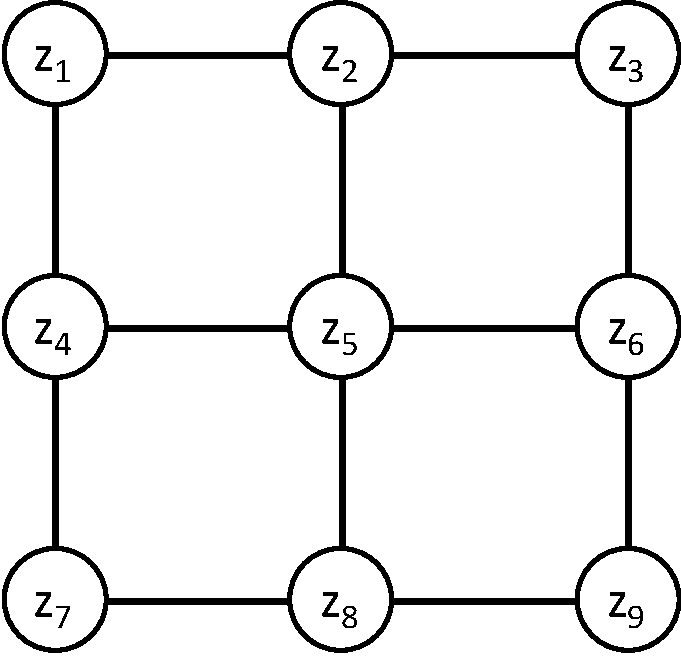
\includegraphics[width=0.2\columnwidth]{c1bi.pdf}
    \vspace{-0.1cm}
  \caption{3$\times$3 image before observing the noise.}
  \label{f:c1bi}
\end{figure}

The node potential is $\phi_i(Z_i)=1$ for each pixel $Z_i=\{0, 1\}$. The edge potential is $\psi_{i,j}(Z_i, Z_j)=\alpha \mathds{1}_{Z_i=Z_j} + \mathds{1}_{Z_i\neq Z_j}$.

The undirected graphical model for 3$\times$3 image after observing the noise is in Figure~\ref{f:c1bii}.
\begin{figure}[h]
  \centering
  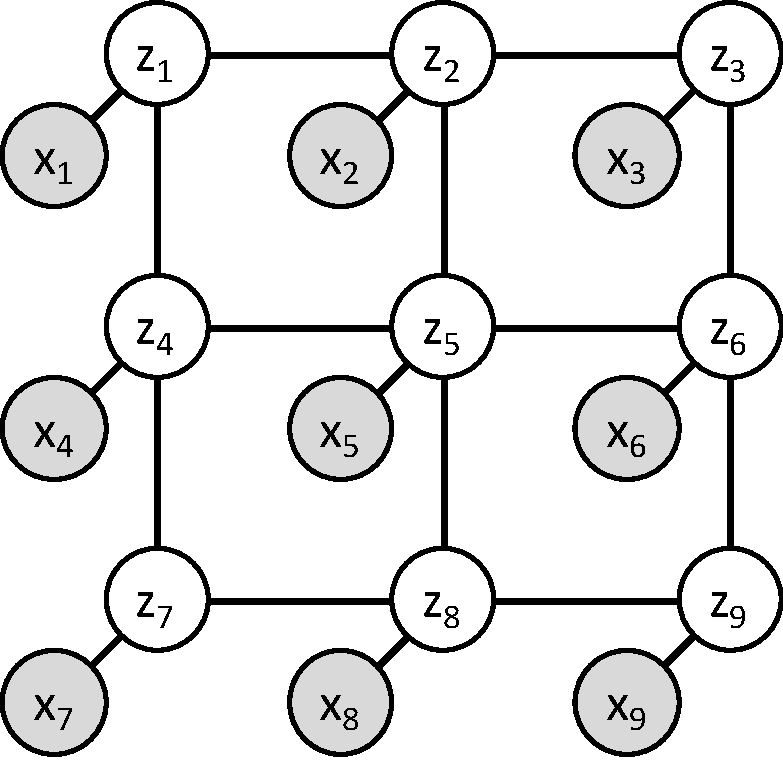
\includegraphics[width=0.2\columnwidth]{c1bii.pdf}
    \vspace{-0.1cm}
  \caption{3$\times$3 image after observing the noise.}
  \label{f:c1bii}
\end{figure}

The shaded node indicates the observed pixel value. The node potential is $\phi_i(Z_i)=1$ for actual value $Z_i=\{0, 1\}$, and $\phi_i(X_i)=\mathds{1}_{X_i = x_i}$ for observed pixel value $x_i$. The edge potential is $\psi_{i,j}(Z_i, Z_j)=\alpha \mathds{1}_{Z_i=Z_j} + \mathds{1}_{Z_i\neq Z_j}$ among actual values $Z$, and $\psi(X_i, Z_i)=(1-\beta) \mathds{1}_{X_i=Z_i} + \beta\mathds{1}_{X_i\neq Z_i}$ between observed and actual pixel values. 
\\

\noindent
(ii) The code for using parallel sum product is
\lstset{language=Python}
\lstset{frame=lines}
\lstset{caption={Using parallel sum product algorithm for photography problem}}
\lstset{label={code:photography}}
\lstset{basicstyle=\footnotesize}
\begin{lstlisting}
import numpy as np
from bp import belief_propagation
from scipy import misc

phi_neutral = {}
phi_neutral[0] = 1
phi_neutral[1] = 1
phi = {0: {}, 1: {}}
phi[0][0] = 1
phi[0][1] = 0
phi[1][0] = 0
phi[1][1] = 1

def save_bmp(img, marginals, file_name):
    array = np.zeros([img.shape[0], img.shape[1]])
    for (i, j) in marginals:
        if i > 0 and j > 0:
            array[i - 1, j - 1] = marginals[(i, j)][0]
    array *= 255
    misc.imsave(file_name, array)


def image_denoise(img, alpha, beta):
    psi_alpha = {}
    psi_alpha[(0, 0)] = alpha
    psi_alpha[(1, 1)] = alpha
    psi_alpha[(0, 1)] = 1
    psi_alpha[(1, 0)] = 1
    psi_beta = {}
    psi_beta[(0, 0)] = 1 - beta
    psi_beta[(1, 1)] = 1 - beta
    psi_beta[(0, 1)] = beta
    psi_beta[(1, 0)] = beta

    node_potential = {}
    edge_potential = {}

    for i in range(1, img.shape[0] + 1):
        for j in range(1, img.shape[1] + 1):
            # node potential for actual value and observation
            node_potential[(i, j)] = phi_neutral
            node_potential[(-i, -j)] = phi[img[i - 1, j - 1]]
            # edge potential for noise
            edge_potential[((i, j), (-i, -j))] = psi_beta
            # edge potential among pixels
            if i - 1 > 0:
                if ((i - 1, j), (i, j)) not in edge_potential:
                    edge_potential[((i, j), (i - 1, j))] = psi_alpha
            if i + 1 <= img.shape[0]:
                if ((i + 1, j), (i, j)) not in edge_potential:
                    edge_potential[((i, j), (i + 1, j))] = psi_alpha
            if j - 1 > 0:
                if ((i, j - 1), (i, j)) not in edge_potential:
                    edge_potential[((i, j), (i, j - 1))] = psi_alpha
            if j + 1 <= img.shape[1]:
                if ((i, j + 1), (i, j)) not in edge_potential:
                    edge_potential[((i, j), (i, j + 1))] = psi_alpha

    marginals = belief_propagation(
        node_potential, edge_potential, diameter=4)

    return marginals


def problem_ii():
    img = misc.imread('./black-white-small-noisy.bmp')
    img[img==255] = 1  # convert to binary
    beta = 0.1
    alphas = [2, 5, 10]
    for alpha in alphas:
        print('alpha', alpha, 'beta', beta)
        marginals = image_denoise(img, alpha, beta)
        save_bmp(img, marginals,
                 './ii_alpha_' + str(alpha) + \
                 '_beta_' + str(beta) + '.bmp')


def problem_iii():
    img = misc.imread('./black-white-small-noisy.bmp')
    img[img==255] = 1  # convert to binary
    alpha = 2
    betas = [0.05, 0.2, 0.4]
    for beta in betas:
        print('alpha', alpha, 'beta', beta)
        marginals = image_denoise(img, alpha, beta)
        save_bmp(img, marginals,
                 './iii_alpha_' + str(alpha) + \
                 '_beta_' + str(beta) + '.bmp')


if __name__ == '__main__':
    print('Problem (ii)')
    problem_ii()

    print('Problem (iii)')
    problem_iii()

\end{lstlisting}
(ii)
The marginal images for problem (ii) are in Figure~\ref{f:denoise_ii}.
\begin{figure*}[t]
\centering
\begin{subfigure}[t]{0.25\textwidth}
  \centering
  \includegraphics[width=\textwidth]{ii_alpha_2_beta_0.1.bmp}
  \vspace{-0.6cm}
  \caption{$\alpha=2, \beta=0.1$.}
  \label{f:ii-1}
\end{subfigure}
\begin{subfigure}[t]{0.25\textwidth}
  \centering
  \includegraphics[width=\textwidth]{ii_alpha_5_beta_0.1.bmp}
  \vspace{-0.6cm}
  \caption{$\alpha=5, \beta=0.1$.}
  \label{f:ii-2}
\end{subfigure}
\begin{subfigure}[t]{0.25\textwidth}
  \centering
  \includegraphics[width=\textwidth]{ii_alpha_10_beta_0.1.bmp}
  \vspace{-0.6cm}
  \caption{$\alpha=10, \beta=0.1$.}
  \label{f:ii-3}
\end{subfigure}
\vspace{-0.3cm}
\caption{Marginal image for problem (ii).}
\label{f:denoise_ii}
\end{figure*}
\\

\noindent
(iii) The marginal image for problem (iii) are in Figure~\ref{f:denoise_iii}.
\begin{figure*}[t]
\centering
\begin{subfigure}[t]{0.25\textwidth}
  \centering
  \includegraphics[width=\textwidth]{iii_alpha_2_beta_0.05.bmp}
  \vspace{-0.6cm}
  \caption{$\alpha=2, \beta=0.05$.}
  \label{f:iii-1}
\end{subfigure}
\begin{subfigure}[t]{0.25\textwidth}
  \centering
  \includegraphics[width=\textwidth]{iii_alpha_2_beta_0.2.bmp}
  \vspace{-0.6cm}
  \caption{$\alpha=2, \beta=0.2$.}
  \label{f:iii-2}
\end{subfigure}
\begin{subfigure}[t]{0.25\textwidth}
  \centering
  \includegraphics[width=\textwidth]{iii_alpha_2_beta_0.4.bmp}
  \vspace{-0.6cm}
  \caption{$\alpha=2, \beta=0.4$.}
  \label{f:iii-3}
\end{subfigure}
\vspace{-0.3cm}
\caption{Marginal image for problem (iii).}
\label{f:denoise_iii}
\end{figure*}
\end{document}